% Solutionary of Programming Evaluations
% Version 1.0, released May 11th. 2018
%
% Author: Jorge Fatama Vera
% Organization: Sociedad de Apoyo para Informáticos (SAI, Society of Support for Informatic Engineers)
% Pontificia Universidad Católica del Perú, Lima, Peru.
% Contact:
% (*) E-mail: jfatamav@e-quipu.pe, jorge.fatama@pucp.edu.pe
% (*) Phone: (+51) 969950140
%
% Licensed by Creative Commmons (CC BY-NC 4.0):
%  (https://creativecommons.org/licenses/by-nc/4.0/)

% DOCUMENT CLASS
% You can change the document characteristics (type, font size, etc), but remember this template was made for articles. [A]
\documentclass[twoside,12pt]{article}
\usepackage{programsol}

% START OF THE DOCUMENT 
\begin{document}                     % Your content begins here.

\AddToShipoutPicture{\BackgroundPic} % Adding the watermark
% The first page doesn't have header and footer
\thispagestyle{empty}
\begin{center}
\begin{large}
    \textsc{\university\\}
    \textsc{\organization\\[0.75cm]}
    \textsc{\course\\}
    \textsc{\evalCourse\space- \currentCycle\\}
    \textsc{Proposed Solution\\}
\end{large}
\end{center}

\section*{Question 1}

\noindent
Lorem ipsum dolor sit amet, consectetur adipiscing elit. Nulla semper congue scelerisque. Lorem ipsum dolor sit amet, consectetur adipiscing elit. Aenean scelerisque magna nec ex fringilla sagittis. Etiam cursus gravida libero sed commodo. Duis tincidunt tortor enim. Nullam rhoncus faucibus leo a facilisis. Maecenas vitae sem pulvinar, feugiat dui eu, cursus massa. Curabitur feugiat semper ipsum, eu dapibus nunc pharetra non. Nunc eu mauris a sem eleifend tempus in nec dolor.\\[0.3cm]

\noindent
Phasellus rutrum eu orci sit amet porttitor. Sed at arcu eu urna accumsan ultricies et sed massa. Donec facilisis metus vitae iaculis posuere. Donec accumsan vel risus eget tempus. Mauris libero elit, ultrices sed mauris in, scelerisque vehicula urna. Sed tempor orci quam, eget convallis elit condimentum non. Phasellus maximus id turpis ac viverra. Sed nec lobortis tellus, ut scelerisque dui. Nam in lectus ipsum. Donec at neque erat.\\

\subsection*{Input}
\noindent
Fusce non sem eu arcu efficitur rhoncus. Nunc nisi ligula, condimentum vel hendrerit in, dapibus nec arcu. Praesent sed sapien commodo augue varius convallis eu sed felis. Fusce ultrices iaculis aliquam. In eleifend est vel hendrerit fermentum. Mauris sollicitudin id nisl eu mollis. Morbi consequat, ipsum et mattis porta, turpis eros aliquet tellus, ut dapibus arcu magna ac diam.

\subsection*{Output}
\noindent
Nulla metus lectus, bibendum ut varius vel, elementum id orci. Etiam ligula nisi, fermentum ac tortor nec, ultricies feugiat quam. Suspendisse leo felis, commodo ac risus eget, tincidunt gravida sapien. Vivamus in risus fermentum purus imperdiet laoreet vel non urna.

\subsection*{Examples}
\noindent
\begin{table}[ht!]
\centering
\label{tbl:tabq1}
\begin{tabular}{|p{6cm}|p{6cm}|}
\hline
\multicolumn{1}{|c|}{\textbf{Input}} & \multicolumn{1}{c|}{\textbf{Output}}  \\ \hline
1            & 1           \\ \hline
2            & 2      \\ \hline
3            & 3           \\ \hline
\end{tabular}
\caption{Some input \& output of the Question 1}
\end{table}

\subsection*{Solution}
{\small
\lstinputlisting[label=cod:p1]{q1.c}
}

\subsection*{Proof}
\begin{center}
    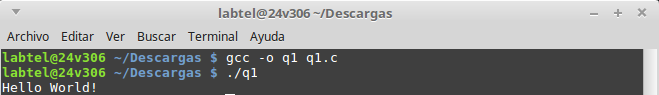
\includegraphics[width=0.6\paperwidth]{scrQ1}
\end{center}

\section*{Question 2}
\noindent
Pellentesque eros odio, viverra vel euismod et, suscipit in odio. Phasellus semper pulvinar convallis. Etiam imperdiet sodales magna, ac scelerisque sapien ullamcorper at. Maecenas sed laoreet velit, a scelerisque augue. Praesent imperdiet, magna id facilisis dapibus, justo nulla placerat sapien, luctus dignissim turpis nibh ut lectus. In non orci quis magna ultricies consequat. Vestibulum posuere vitae elit in dignissim. Nulla eget nulla eu tellus pulvinar pellentesque quis ut leo. Ut cursus sapien ut velit ornare pellentesque. Nulla facilisi. Suspendisse ante libero, luctus in condimentum tincidunt, ultricies at orci. Nulla eleifend est nec metus convallis consequat commodo a risus. Etiam sit amet tempus mauris, eu malesuada metus. Praesent quis tempus felis. Donec in auctor diam.

\begin{equation}
    \Large \int_{a}^{b} x^n dx = \frac{(a^{n+1}-b^{n+1})}{n+1}
\end{equation}

\subsection*{Input}
\noindent
Sed id massa leo. Pellentesque placerat egestas sapien nec viverra. Orci varius natoque penatibus et magnis dis parturient montes, nascetur ridiculus mus. Sed tempor, quam non egestas lobortis, risus eros maximus augue, condimentum hendrerit ante ipsum eget est. Integer quis elementum tellus, et pulvinar sapien. Morbi cursus scelerisque metus, id aliquam eros gravida eget.\\[0.3cm]
Curabitur posuere elit tellus, eu egestas ante finibus a. In luctus nibh consectetur, gravida sem a, volutpat sapien.

\subsection*{Output}
\noindent
Quisque finibus ligula sodales elit congue pharetra quis nec nisl. Nullam tristique fermentum elit vel mollis. Sed commodo sapien ac tortor blandit, non pulvinar purus ullamcorper. Suspendisse at justo eu est venenatis vestibulum consectetur nec ipsum. Proin malesuada erat vel malesuada maximus. Maecenas sodales vehicula massa, non tempus neque tristique semper. Donec in ex venenatis, tincidunt velit at, vulputate enim.\\[0.3cm]
Mauris pharetra volutpat mi sed tempor. Interdum et malesuada fames ac ante ipsum primis in faucibus. Mauris eget commodo dui. Nulla nec iaculis purus. Mauris pharetra lacinia dapibus. Donec massa mauris, pretium vel rutrum nec, congue eleifend dolor. Nam varius dui ut pellentesque ornare. Maecenas sed nisl quam. Vivamus pulvinar facilisis eros, sit amet fringilla ex rutrum at. Praesent consectetur lectus enim, et pretium nunc pretium non.

\subsection*{Examples}
\noindent
\begin{table}[ht!]
\centering
\label{tbl:tabq2}
\begin{tabular}{|p{6cm}|p{6cm}|}
\hline
\multicolumn{1}{|c|}{\textbf{Input}} & \multicolumn{1}{c|}{\textbf{Output}}  \\ \hline
n a b       & \Large $\frac{(a^{n+1}-b^{n+1})}{n+1}$           \\ \hline
2 4 3       & -12.33      \\ \hline
5 1 4       & 682.50           \\ \hline
\end{tabular}
\caption{Some input \& output of the Question 2}
\end{table}

\subsection*{Solution}
{\small
\lstinputlisting[label=cod:p2]{q2.c}
}

\subsection*{Proof}
\begin{center}
    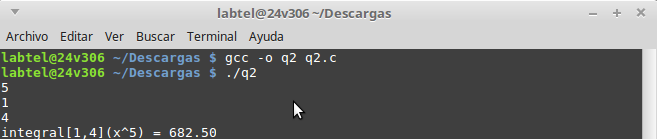
\includegraphics[width=0.6\paperwidth]{scrQ2}
\end{center}

\begin{flushright}
    \footnotesize{Format based on Template \textit{Solutionary of Programming Evaluations}, by Jorge Fatama Vera (SAI PUCP)}\\
\end{flushright}

\end{document}                      % Your content finishes here.
% END OF THE DOCUMENT

% References:
%
% in main.tex
% [A] List of available document classes: https://tex.stackexchange.com/questions/782/what-are-the-available-documentclass-types-and-their-uses
%
% in programsol.sty
% [1] babel Documentation: http://ctan.uniminuto.edu/macros/latex/required/babel/base/babel.pdf (in page 18, you can see the list of available languages in babel).
% [2] inputenc Documentation: http://ctan.uniminuto.edu/macros/latex/base/inputenc.pdf
% Watermark guide: https://tex.stackexchange.com/questions/256750/transparent-textbox-behind-text-on-title-page
% [3] Headers & Footers Guide: https://en.wikibooks.org/wiki/LaTeX/Customizing_Page_Headers_and_Footers
% [4] eso-pic Documentation: http://ctan.uniminuto.edu/macros/latex/contrib/eso-pic/eso-pic.pdf
% [5] Listing Format Guide: https://en.wikibooks.org/wiki/LaTeX/Source_Code_Listings